\chapter{POI空间数据分析}{Spatial Data Analysis of Weibo POIs}
新浪微博签到是新浪微博用户在使用移动终端发送微博时,使用移动终端的定位功能,
用户可以选择附近热门的位置或者自行添加位置的功能\cite{韩华瑞2016湖北省微博签到活动空间差异分析——以新浪微博为例}。
这些位置信息将会被存储到新浪微博数据服务器中,在微博网页端,可以查看该签到位置的详细信息,这些签到数据称为
感兴趣点POI(Point Of Interest)\cite{Ye2011Exploiting},见图\ref{fig:webpoi}。
\begin{figure}
  \centering
  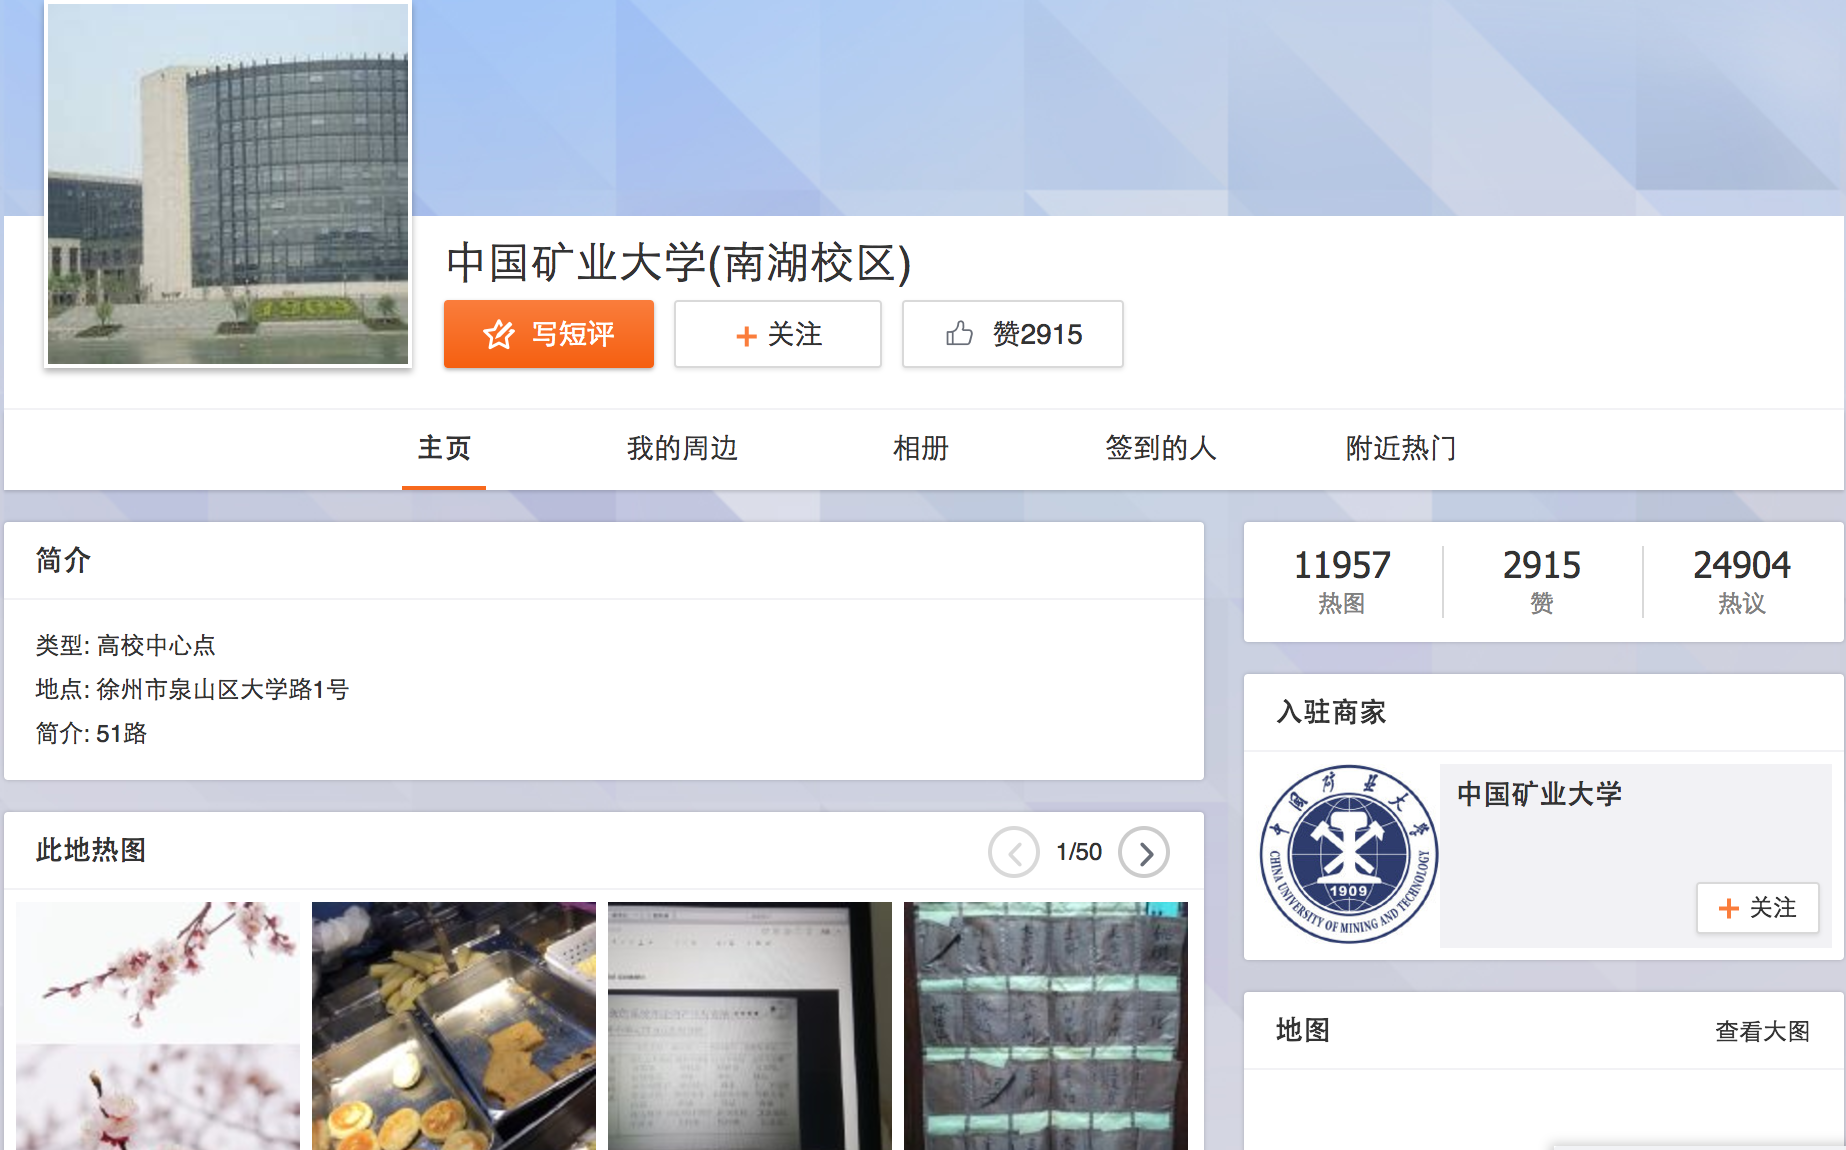
\includegraphics[width=10cm]{figures/webpoi.png} \ \
  \caption{微博网页POI}{POI in web}
  \label{fig:webpoi}
\end{figure}


\section{POI数据获取}{POI Data Fetch}

新浪微博提供了place/nearby/pois接口获取附近的POI数据,该接口参数见表\ref{tab:api_poi}。
\begin{table}
  \centering
  \caption{POI接口参数(部分)}{POI api parameters(partly)}
  \label{tab:api_poi}
  \tabulinesep=1.5mm
  \begin{tabu}to 0.8\linewidth{X[0.8,c]X[1,c]X[1,c]X[2.8,c]}
    \tabucline[0.1em]-
    接口 & 参数 & 类型 & 说明 \\
    \tabucline-
    \multirow{3}{*}{POI} & lat & Float & 纬度 \\
      & long & Float & 经度 \\
      & range & Int & 查询半径,最大10km \\
    \tabucline[0.1em]-
   \end{tabu}
\end{table}

为了获取全国范围内POI数据,需要对全国区域内进行「地毯」式查询,而上述新浪微博
API接口的坐标参考系统是不一致的,查询点经纬度属于椭球坐标系统(大地坐标系统),
而查询半径属于平面坐标系统(投影坐标系统),因此需要针对查询坐标进行一步预处理。

(1)投影:
地图投影多种多样,按照某种特定的要求地图投影可分为等角投影、等距投影和等积投影\cite{Yang1999Map},
我国常用的投影是高斯投影,但高斯投影存在离中央经线越远,变性越大等缺点,而且需要划分较多的投影带,
处理较为繁琐。
	
Lambert投影属于等角圆锥投影,通过投影圆锥面割于椭球体面的两纬线,减少南北方向的变形。Lambert
投影主要用于南北方向跨度较大的地区成图,我国绝大多数省(区)位于中纬地区,因此采用Lambert
正轴等角割圆锥投影,参数为中央经度为$105^{\circ}\text{\textrm{E}}$,第一标准纬度$25^{\circ}\text{\textrm{N}}$,
第二标准纬度为$47^{\circ}\text{\textrm{N}}$

(2)栅格化:
为了实现「地毯」式搜索,需要将投影后的全国边界面要素进行栅格化处理,
由于新浪微博API在查询半径上限为$10\text{\textrm{km}}$,为了减少查询次数,
设计方案如图\ref{fig:grid},栅格化的大小为$10/\sqrt{2} \times 2 =10\sqrt{2}=14.1\text{\textrm{km}}$
\begin{figure}
\centering
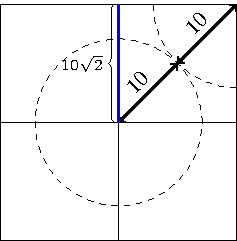
\includegraphics[scale=0.8]{figures/query.pdf}

\caption{查询示意图}{Query illustration}
\label{fig:grid}
\end{figure}

(3)投影坐标反算:
栅格化后,每个点坐标为投影平面坐标系,为了与新浪微博API接口匹配,需要将查询点的平面
坐标通过Lambert投影反算,转换成经度和纬度(椭球坐标)。

本文使用新浪微博C\# SDK开发了新浪微博数据获取应用程序,启动程序后,登录新浪微博账号,
程序向新浪微博授权服务器获取授权后,获得调用新浪微博API的权限。
为了防止频繁访问服务器而导致返回不全数据或者空数据,需要在每次完成请求后线程暂停数毫秒,同时为了
能够多进程并发执行,将查询点拆分为若干个文件,程序界面见图\ref{fig:crawler},每个进程使用一份查询点文件。
\begin{figure}
  \centering
  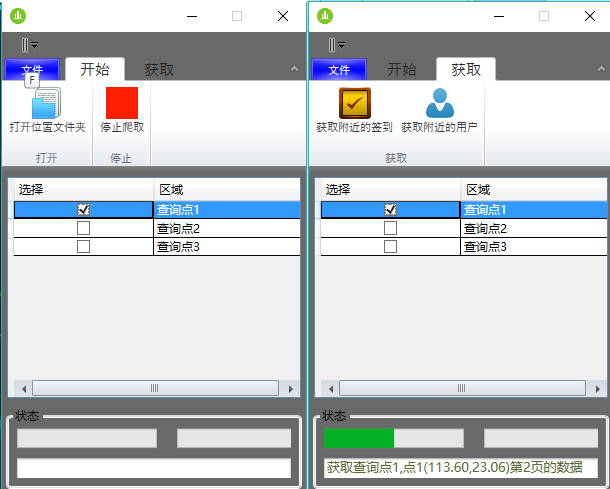
\includegraphics[width=8cm]{figures/crawler.png} \ \
  \caption{程序界面}{Program interface}
  \label{fig:crawler}
\end{figure}

这些POI包含了位置、类别、签到数目等数据,见表\ref{tab:propertiesofpoi}。
\begin{table}
  \centering
  \caption{新浪微博POI数据(部分)}{Properties of Weibo POI(partly)}
  \label{tab:propertiesofpoi}
  \tabulinesep=1.5mm
  \begin{tabu}to 0.9\linewidth{X[1,c]X[1,c]|X[1,c]X[1,c]}
    \tabucline[0.1em]-
    属性 & 说明 & 属性 & 说明 \\
    \tabucline-
    PID & POI编号 &  Name & POI名称  \\
    Longitude & POI经度 & Latitude & POI纬度 \\
    Category & POI类别 & CheckNumber & POI签到数量  \\
    \tabucline[0.1em]-
   \end{tabu}
\end{table}

新浪微博返回的数据为JSON格式,表\ref{tab:propertiesofpoi}中的每个属性值都是以key$-$value形式
保存在JSON文本中,但是由于网络或者新浪服务器等问题,有些JSON记录数据不全,噪声较多,因此这些数据不适宜保存
在传统的关系型数据库中,因为数据库表的结构需要在使用前定义,因此将获取的$900$多万条微博POI,共$2.3$G
数据按行存储到HDFS中。

\section{统计分析}{Statistical Analysis}
Spatial-Spark不仅仅支持空间数据,对于非空间数据处理仍然保留了Spark计算框架的接口,Spark RDD提供了丰富
的操作如合并(Union),去重(Distinct),过滤(Filter)等操作,方便开发者使用。

\subsection{热门签到地点}
每个POI数据都包含了签到数量,在RDD中使用sortBy和take操作,通过简单的排序,可以获取签到数
量前10位的POI,详细内容见表\ref{tab:top10poi}。
\begin{table}
  \centering
   \caption{热门签到地点}{Hottest POIs in top 10}
   \label{tab:top10poi}
  \tabulinesep=1.5mm
  \begin{tabu}to 1.0\linewidth{X[1.7,c]X[1.5,c]|X[1.7,c]X[1.5,c]}
    \tabucline[0.1em]-
    POI名称 & 签到数量 & POI名称 &  签到数量 \\
    \tabucline-
    星光公益站  & $399622$ & 丽江古城  & $160032$ \\
    浦东机场  & $184263$ & 成都双流国际机场 & $158121$ \\
    厦门高崎国际机场  & $181911$ & 望京  & $148109$ \\
    中关村 & $166640$ & 首都机场T$3$航站楼  & $140470$ \\
    深圳宝安国际机场& $162857$ & 广州白云机场 & $136998$ \\
    \tabucline[0.1em]-
   \end{tabu}
\end{table}

\subsection{热门签到类别}
每个POI数据也包含了该POI所属的类别,使用RDD的groupBy和reduceByKey两个算子,统计出每个POI类别
的数量,以新浪微博Logo制作出POI类别词云,见图\ref{fig:poiwordclound},词条频数越大,词条字体越大。
从图中可以看出生活娱乐类别是新浪微博POI类别中数量最多的,从侧面说明了新浪微博POI对人活动信息的反映,
而这些信息对商家的广告投放、微博旅游推荐\cite{朱晨曦2016基于微博签到的地理空间信息研究}有重要的参考意义。
\begin{figure}
  \centering
  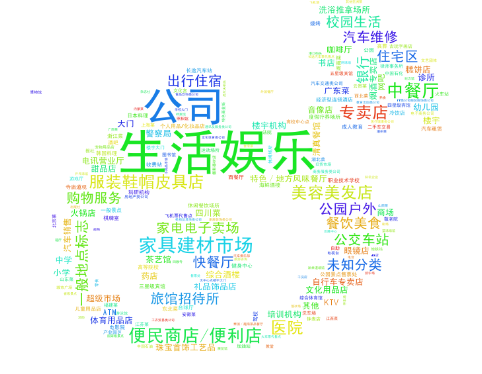
\includegraphics[width=7cm,height=5.25cm]{figures/poi_category.png} \ \
  \caption{POI类别词云}{Word cloud of pois' category}
  \label{fig:poiwordclound}
\end{figure}

\section{同位模式}{Co-Location Pattern}
频繁模式是频繁出现在数据集中的模式\cite{Agrawal1995Mining},一般认为频繁模式中的项与项之间存在
一定的相关性,同时它们之间也存在推导规则,根据一定算法可以发现事物之间关系并进行预测\cite{Agrawal1999Automatic}。
目前空间关联分析可以划分为单主题和多主题的两种模式,单主题空间模式发现是传统关联分析在空间维度上拓展,
但是存在人工干预等缺点;多主题模式单纯地寻找在空间聚集一起的事物,也就是空间空位模式(co-location pattern)。

\subsection{关联规则算法}
关联规则是无监督机器学习领域中研究最活跃、最广泛的一种算法\cite{王佐成2006空间关联规则的双向挖掘},通过对数据库
记录进行多次扫描,就可以获得非常简单的表述形式。而且关联规则也非常容易解释,数学模型描述如下:

假设事务项(Transaction)为$T$,每个事务项$T$都是由集合$I={I_1,I_2,\ldots,I_m}$组合而成,其中集合$I$中项(Item)各不相同。
$P$为项$I_i$的一个组合,如果$P$属于$T$,
则称事务$T$包含$P$,那么关联规则的表达形式是$P \rightarrow Q$,其中$P\in T, Q\in T$并且$P \cap Q=\emptyset$。
关联$P \rightarrow Q$在数据集$D$中成立,需要满足支持度$s$和置信度$c$的
约束\cite{陈江平2004空间关联规则挖掘算法研究}。置信度是事务集$D$中包含组合$P$又包含组合$Q$的百分比;支持度是
组合$P$出现的事务中,包含组合$Q$事务的百分比\cite{蔡伟杰2001关联规则挖掘综述}。

在这里定义强规则是指既要不小于支持度阈值($min\_s$)又不小于置信度阈值$min\_c$的规则,如果 
$s(P\rightarrow Q) \ge min\_s$,则称$P\cap Q$是频繁项集;如果$c(P\rightarrow Q) \ge min\_c$,则称
规则$P\rightarrow Q$成立。

关联规则挖掘算法中最著名要属Agrawal R.和Srikant R.在提出的布尔规则关联频繁集合算法(Apriori算法)
\cite{Koperski1995Discovery},该算法的核心思想为两条:\circled{1}频繁项的子集必须也是
频繁的;\circled{2}非频繁项的超集必定非频繁。因此Apriori算法主要分为两个步骤:

(1)连接步

$L_{k-1}$自相连产生$k$项集的生成$C_k$,再通过$C_k$筛选出$L_k$。根据Apriori算法第二个条件,
在生成$L_k$集合过程中,可以避免一些非频繁项连接。

(2)剪枝步

如果所有的频繁$k$项集都包含在$C_k$中,但$C_k$中的成员却不一定全是频繁的。通过Apriori算法的
第一个条件,如果某$k$项集中存在非频繁项,那么该$k+1$项必定非频繁,可将其删除做剪枝处理。

\subsection{单主题空间关联规则}
Koperski K.将传统的关联规则挖掘拓展至空间关联规则挖掘,单主题空间关联规则研究得到了
广泛的关注和研究。单主题的空间关联规则挖掘以某一类空间实体展开\cite{Ester1999Spatial},
发现周边其他类别的空间实体与其关系。

实体之间的关系可分为非空间谓词和空间谓词,非空间谓词表示空间对象的非空间的性质的谓词,如价
格、种类、颜色等;而空间谓词则表达空间对象由于空间对象位置而形成的相互之间的联系,一般来讲
分为空间拓扑关系、空间距离关系和空间方位关系。典型的的空间关联规则如式\eqref{eq:spaitalrelation}
所示,其中$P_i$和$Q_j$中至少有一个为空间谓词。
\begin{equation}
\label{eq:spaitalrelation}
P_1\wedge P_2\wedge \ldots \wedge P_m \rightarrow Q_1\wedge Q_2\wedge \ldots \wedge Q_n(s\%, c\%)
\end{equation}

当空间对象分布不均匀的时候,单主题空间关联规则会出现关注对象不突出,不利于反映真实的空间关联性。
改进的算法有基于$k$邻近的空间关联模式挖掘\cite{万幼2008k},该算法优化了空间关系选择方案,选择空间
$k$个近邻对象,然后建立空间关系事务项,使用经典的关联规则算法进行数据挖掘。该算法呢通过选择$k$个近邻
空间对象,避免的空间对象分布不均匀的问题,但是该算法需要指定$k$值,$k$值过小,空间关系表现非常匮乏,而
$k$值过大,将会导致空间事务项阶数激增,关联关系噪声较大\cite{Bian2009A}。

\subsection{多主题同位模式}

传统的数据通常是相互独立的,而空间上分布的对象则是相关的,也就是空间并置(co-located),即两个对象位置
越近,就越有可能有相似的性质或者有较强的相关性。Shekhar S.等人提出了基于空间相关的同位模式分析\cite{Jin2006A},即主题的空间关联规
则。该模型将事务概念泛化,以一定距离领域范围包含的空间对象作为空间关联规则的事务,提出空间实体分布的同位模式,并且很好
地考虑到空间实体之间的相关性\cite{Huang2004Discovering}。

一般来讲,距离越近的空间对象越具有相关性,因此同位模式选择特定的距离作为判断空间对象关联依据,并且将其
以事务表项保存。以图\ref{fig:spaitalrelation}为例,空间范围内有个$A,B,C$三类事物,包含了
$a_1,a_2,a_3,a_4,b_1,b_2,b_3,b_4,b_5,c_1,c_2\text{和}c_3$空间实体对象,空间邻近关系$R$定义为两个
空间实体对象之间的距离不大于距离$d$,见式\eqref{eq:colation},如果满足空间邻近关系$R$则将空间对象连接起来。

\begin{figure}
\centering
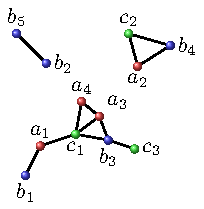
\includegraphics[width=0.3 \linewidth]{figures/spatialrelation.pdf}
\caption{空间关系示意图}{Spatial relation illustration}
\label{fig:spaitalrelation}
\end{figure}
\begin{equation}
\label{eq:colation}
 R(a_1,b_1) \Leftrightarrow (distance(a_1,b_1)\le d)
\end{equation}

空间特征集代表了空间不同种类对象的集合,记为$F=\{f_1,f_2,\ldots,f_n \}$;每一个具体空间位置上的对象称之为空间实例;
空间实例集$I=\{I_1,I_2,\ldots,I_m\}$,如果有$\{R(I_j,I_k) | 1 \le j \le m, 1 \le k \le m\}$,称$I$为一个簇;
空间co-location模式是一组空间特征的集合$C$,其中$C\in F$,一个co-location模式$C$的长度称此co-location的阶(Order);如果簇$I$的
包含了co-location模式$C$中的所有特征,并且$I$中没有任何一个子集可以包含$C$中所有特征,那么称$I$就是co-location模式$C$的
一个行实例$row\_instance(C)$,co-location的所有行实例表示为一个表实例$table\_instance(C)$。

在图\ref{fig:spaitalrelation}中,空间特征集为$F=(A,B,C)\text{,而}\allowbreak (c_2,b_4,a_2),\allowbreak (a_3,c_1,b_3)\text{,} \allowbreak (a_1,b_1) \text{,} \allowbreak (a_1,c_1)\text{,} \allowbreak (c_1,a_4)\text{和}(b_3,c_3)$
表示为一个簇。$(A,B,C)$可以表示为一个co-location模式,$(a_2,b_4,c_2)\text{和}(a_3,c_1,b_3)$表示了该co-location的行实例,
所有的行实例将组成表实例。

参与率和参与度是衡量co-location模式挖掘中重要参数,反映了一个空间模式的频繁程度。

(1)参与率

设$f_i$为某个空间特征,$f_i$在$k$阶co-location模式$C$中的参与率(participation ratio)表示为$PR(c, f_i)$,它是$f_i$的实例
在空间co-location模式$C$的所有不重复实例中不重复出现的个数与总实例的比例,定义见式\eqref{eq:participateratio}。
\begin{equation}
\label{eq:participateratio}
PR(c,f_i)=\frac{|\pi_{f_i}(table\_instance(c))|}{|table\_instance(\{f_i\})|}
\end{equation}

例如图\ref{fig:spaitalrelation}中,同位模式$(A,B,C)$所有的实例为$(a_2,b_4,c_2)\text{和}(a_3,c_1,b_3)$,空间特征$A$的实例对象
有$2$个$(a_2,a_3)$,而空间特征$A$的所有实例有$4$个$(a_1,a_2,a_3,a_4)$,所以$PR(\{A,B,C\},A)=2/4=0.5$;同理
$PR(\{A,B,C\},B)=2/5=0.4$,$PR(\{A,B,C\},C)=2/3=0.67$。

(2)参与度

co-location模式$c=\{f_1,f_2,\ldots,f_k\}$的参与度(Participation Index)表示为$PI(c)$,它是co-location
模式$C$的所有空间特征的$PR$值中的最小值,定义见式\eqref{eq:participateindex}
\begin{equation}
\label{eq:participateindex}
PI(c)=min_{i=1}^{k}\{PR(c,f_i)\}
\end{equation}

图\ref{fig:spaitalrelation}中,$PI(\{A,B,C\})=min(0.5,0.4,0.67)=0.4$。

$min\_prev$是需要给定的最小参与度阈值,只有当$PI(c) \ge min\_prev$时,称co-location模式$C$是频繁的。
co-location算法主要是基于最小参与度,由于最小参与度概念与Apriori算法相同的性质(向下闭合),很大程度上能降低
算法复杂度的开销,此类算法研究主要有:

\circled{1}Join-Based算法:一种基于完全连接的算法。该算法严格使用Apriori算法,$k$阶模式表之间通过连接(Join)操作
生成$k+1$阶候选者,对$k+1$表实例按照最小参与度筛选,该算法能够产生完整的co-location模式。

\circled{2}Partition-Join算法:一种基于部分连接的算法。该算法采用分治的思想,首先把空间所有按照距离阈值划分为不相交的实体块,
块与块之间实体不满足空间关联性,这样只需要进行块内部空间对象连接,大大降低了连接的计算量\cite{Yoo2004A}。算法的关键之处如何很好划分
出空间实体块,降低复杂度。

\circled{3}CPI-Tree算法:一种基于前缀树结构的无连接改进算法\cite{Wang2009Efficient}。该算法以前缀树表达空间实体对象之间的邻近关系,通过树结构
可以快速地处理表实例的增长,拥有较高的性能。但是如果数据量较大,存储和遍历树的代价将会增加,是一种折中的解决方案。

\subsection{Spatial-Spark同位模式}

全连接算法是一个依据先验原理,基于Join-Based操作产生候选模式和表实例的方法。主要流程分为以下两步:

(1)候选行实例生成

连接两个$k-1$个空间对象相同的频繁$k$阶模式实例表$P_{k1}$和$P_{k2}$,
生成$k+1$阶的候选行实例,在生成的过程中,检查行实例的所有对象是否满足空间距离阈值$d$。

(2)表实例的生成

根据所有候选行实例,按照每个行实例的模式进行汇总形成候选表实例,
对每个表实例计算所有特征的参与度,按照参与度过滤不满足阈值的表实例。

算法过程中,首先需要进行二阶模式行实例和表实例生成,算法时间复杂度将达到$O(n^2)$,当数据量急剧增加时候,
算法的时间消耗是不可接受的,需要进行并行化处理。借鉴Spatial-Spark计算框架中的空间连接运算,根据空间同位模式
的距离阈值$d$,将整个平面空间位置划分为均匀网格。以空间对象落入网格的横纵坐标编号作为
空间实体的Key,将所有空间实体生成Key-Value形式,见图\ref{fig:twoorder}中\uppercase\expandafter{\romannumeral1}
所示,每个空间实体对象拥有唯一的坐标。
\begin{figure}
\centering
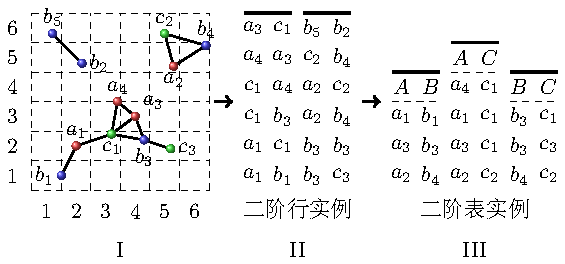
\includegraphics[width=0.8 \linewidth]{figures/two_order.pdf}
\caption{二阶模式生成}{Generation of 2 order location pattern}
\label{fig:twoorder}
\end{figure}

紧接着对所有实体对使用cogroup算子进行自相连,生成所有满足距离阈值的空间实体对,为了完整得获取所有空间邻近关系,
对坐横纵坐标差值绝对值不大于$1$的空间实体可判定为在可能存在邻近关系,
图\ref{fig:keyequal}中\uppercase\expandafter{\romannumeral1}, \uppercase\expandafter{\romannumeral2}
和\uppercase\expandafter{\romannumeral3}分别表示了三种相等情况。再使用filter算子进行过滤判断严格的邻近关系,
经过mapToPair操作生成所有的行实例,最后使用reduce操作按空间参与度过滤生成表实例。
\begin{figure}
  \centering
  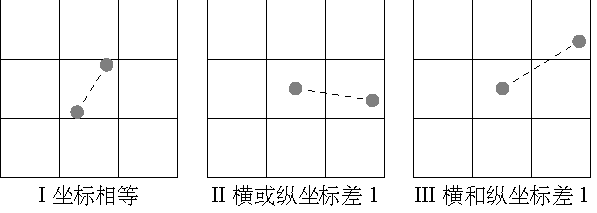
\includegraphics{figures/keyequal.pdf}
  \caption{坐标相等判断}{Judgement of coordinate equality}
  \label{fig:keyequal}
\end{figure}

图\ref{fig:twoorder}展示了完整的二阶生成模式流程,
\uppercase\expandafter{\romannumeral2}为列出所有行实例,\uppercase\expandafter{\romannumeral3}
则按照空间实体的特征进行汇总,按照参与度进行剪枝操作。
生成二阶模式后,根据同位模式的连接和剪枝步骤,生成更高阶数同位模式,见算法\ref{alg:colocaiton}。
% \begin{figure}
% \centering
% 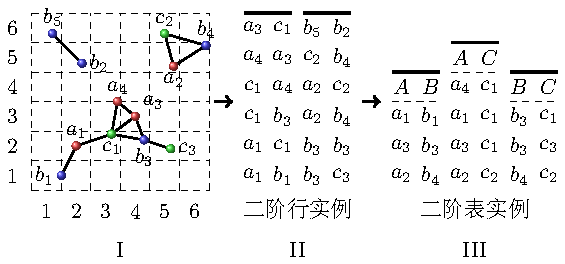
\includegraphics[width=0.8 \linewidth]{figures/two_order.pdf}
% \caption{二阶模式生成}{Generation of 2 order location pattern}
% \label{fig:twoorder}
% \end{figure}
\begin{algorithm}
\caption{co-location算法}
\label{alg:colocaiton}
\begin{algorithmic}[1]   
\REQUIRE  ~~\\  
点集:points;\\  
距离阈值:d;\\
参与度阈值:threshold;\\  
\ENSURE ~~\\  
空间同位模式:colocation patterns; \\
\STATE $P_2$ = Spatial-Spark.join(points, d, threshold)
\WHILE{$P_k$ is not empty and $k$ < N} 
\STATE $C_{k+1}$ = gen\_candinate\_cocolation($P_k$,$k$) $//$k+1阶候选集合
\STATE $C_{k+1}$ = pruning($C_{k+1}$, $d$) $//$剪枝处理
\STATE $T_{k+1}$ = gen\_table\_ins()$//$生成表实例
\STATE $P_{k+1}$ = Select\_Colocation\_Pattern($T_{k+1}$, threshold) $//$ 筛选表实例
\STATE $k$ = $k+1$ $//$下一轮迭代
\ENDWHILE 
\RETURN $P_2$,$\dots$,$P_k$
\end{algorithmic}  
\end{algorithm}

为了将不同的表实例进行连接操作,需要重写Join操作中key相等判断操作,定制了RowPattern类,重写equal方法,
当且仅当只有一个空间实例不等的时候,该行实例才相等。

RDD提供了Join操作,该操作对每个key下元素进行笛卡尔乘积,返回的结果再展平。当对$k$阶行实例进行join操作后,
对新加入的新添加的POI对象进行距离阈值$d$判断,获得有效的$k+1$阶行实例。以行实例的POI的类别Pattern为key进行
reduce操作生成表实例,按照参与率阈值进行剪枝操作,生成$k+1$阶表实例。设$k$阶模式$C1$和$k$阶模式$C2$连接得到$k+1$阶
候选模式$c3$,$C1$的行实例个数为$K1$,$C2$的行实例的个数为$K2$,$C3$的行实例个数为$K3$,在算法过程
中对$C1$和$C2$表进行连接操作,之后再$C3$表中进行查找,整个算法时间复杂度$O((k-2)K1\times K2 \times K3)$,实现
过程如下。
\begin{lstlisting}[language=Java][H]
while(colocations.count!=0){
  JavaPairRDD<RowPattern,Iterator<POI>> 
      rawRowInstances=colocations.join(colocations);
  JavaPairRDD<RowPattern,Iterator<POI>>
      validRowInstances=rawRowInstances.filter(
        //距离阈值判断
        distanceThresholdCheck();
      )
  JavaPairRDD<Pattern,Iterator<Iterator<POI>>>
      validTableInstance = validRowInstances.reduceBykey(
        //按pattern合并行实例
        combineRowInstances();       
      ).filter(
        //按照参与度进行剪枝
        participateratioCheck();
      );
  colocations=validTableInstance.mapToPair(
      //展开下一阶行实例
      flatRowInstances();
  )
}
\end{lstlisting}


\section{微博POI同位模式}{Co-Location Patterns in Weibo POIs}

微博用户签到地点是非常有趣的数据,反映了新浪微博用户在线下的活动情况,对现实生活的商圈发现、地点推荐
等重要的参考依据。POI空间模式挖掘中,为了过滤掉噪声信息,需要经过两步预处理:\circled{1}过滤签到数量较少的POI,
选择签到数量大于10的POI点;\circled{2}过滤POI所属类别不清楚,如「一般地点」、「楼宇」和「大门」等。

\subsection{二阶同位模式识别}
以不同的城市为研究区域,探索不同城市微博POI空间模式分布特征。选择空间距离阈值$d=500\text{\rm{m}}$,上海、武汉和
重庆三市微博POI类别二阶特征模式。由于新浪微博POI类别分类并非严格区分,比如「餐饮美食」与「中餐厅」存在着包含关系,因此
我们选择某一类别进行重点关注,比如选择「高等院校」在新浪微博POI中的与其他类别的同位关系及其空间参与度,
见表\ref{tab:advanceacademic}。
\begin{table}
  \centering
  \caption{高等院校二阶同位模式}{Advance academics' 2-order patterns}
  \label{tab:advanceacademic}
  \tabulinesep = 1.5mm
  \begin{tabu}to 1.0\linewidth{X[1,l,m]|X[1,l,m]| X[1,l,m]}
  \tabucline[0.1em]-
  \rowfont[c]{} 上海市 & 武汉市 & 重庆市 \\
  \tabucline-
  (高等院校,校园生活):0.556 &  (高等院校,校园生活):0.531 & (高等院校,校园生活):0.306 \\
  (高等院校,日本料理):0.472 & (高等院校,图书馆):0.528 & (高等院校,ATM):0.238 \\
  (高等院校,西餐厅):0.454 & (高等院校,糕饼店):0.384 & (高等院校,科研机构):0.224 \\
  (高等院校,甜品店):0.451 & (高等院校,快餐厅):0.368 & (高等院校,图书馆):0.224 \\
  (高等院校,培训机构):0.446 & (高等院校,四川菜):0.361 & (高等院校,超市):0.217 \\
  (高等院校,医院):0.443 & (高等院校,火锅店):0.358 & (高等院校,特色餐厅):0.215 \\
  (高等院校,糕饼店):0.441 & (高等院校,连锁酒店):0.354 & (高等院校,电子卖场):0.210 \\
  (高等院校,餐饮美食):0.432 & (高等院校,医院):0.328 & (高等院校,KTV):0.205 \\
  \tabucline[0.1em]-
  \end{tabu}
\end{table}

从表\ref{tab:advanceacademic}可以看出上海、武汉和重庆三市高等院校与周边同位模式POI类别差别不大,都是
与高校配套的相关服务类型,但是每个城市高等院校的周边类别差异较大。
由于上述三城市高等院校数量依次减少,因此相应的空间模式的空间参与度呈现下降趋势。

以(高等院校,培训机构)二阶模式为例,研究在不同空间距离阈值条件下在上述三市中空间参与度分布情况,
见图\ref{fig:participationIndexes},随着距离阈值增大,同位模式的空间参与度逐渐上升,而不
不同城市之间差异也非常明显。
\begin{figure}
  \centering
  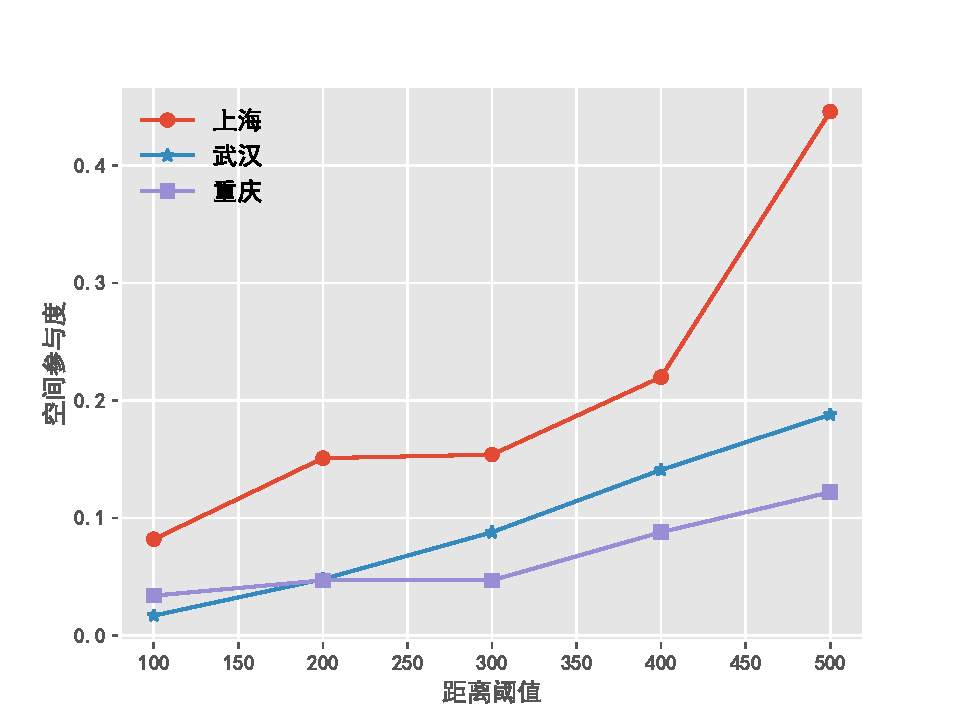
\includegraphics[scale=0.8]{figures/Participate.pdf} \\
  \caption{(高等院校,培训机构)模式不同距离阈值在不同城市空间参与度}{(Academic institutions \& Training institutions) Pattern's Paticipation indexes in different distances and cities}
  \label{fig:participationIndexes}
\end{figure}

\subsection{高阶同位模式识别}
北京市是全国新浪微博POI数量最多的城市,对该城市的新浪微博POI进行空间同位模式更具有代表性。在空间同位模式挖掘算法中,
连接距离阈值$d$和参与度阈值threshold是两个非常重要的,不同的参数将生成不同的空间同位模式,因此不同参数对北京市的POI进行
空间同位模式挖掘结果见表\ref{tab:distanceandthreshold}。
\begin{table}
  \centering
  \caption{不同距离和参与率空间同位模式}{Co-location patterns in defferent distances and PI's thresholds}
  \label{tab:distanceandthreshold}
  \tabulinesep=1.5mm
  \begin{tabu}to 0.8\linewidth{X[1.3,c,m]X[1.5,c,m]X[1,c,m]X[1,c,m]X[1,c,m]X[1,c,m]X[1,c,m]}
    \tabucline[0.1em]-
    距离\par 阈值 & 参与率 \par 阈值 & 2阶 & 3阶 & 4阶 & 5阶 & 6阶 \\
    \tabucline-
    \multirow{3}{*}{300} & 0.5 & 9 & 4 & 1 & - & - \\
     & 0.6 & 8 & 2 & - & - & - \\
    	& 0.7 & 5 & 1 & - & - & - \\
    \tabucline-
    \multirow{3}{*}{400} & 0.5 & 23 & 22 & 13 & 3 & - \\
     & 0.6 & 17 & 9 & 2 & - & - \\
     & 0.7 & 11 & 3 & - & - & - \\
    \tabucline-
    \multirow{3}{*}{500} & 0.5 & 40 & 40 & 26 & 11 & 2 \\
      & 0.6 & 29 & 29 & 19 & 7 & 1 \\
     & 0.7 & 22 & 17 & 7 & 1 & - \\
    \tabucline[0.1em]-
   \end{tabu}
\end{table}

通常来讲,距离阈值越大,参与率阈值越小,空间模式的生成阶越大,每一阶的模式数目越多。本文选择$d=500\text{\rm{m}}$,
参与度阈值为$0.6$,该参数既可以保留足够的细节信息,又能较好地反应空间分布的整体特征\cite{禹文豪2015设施},
新浪微博微博POI空间同位模式见表\ref{tab:poilocationpattern}。
\begin{table}
  \centering
  \caption{POI空间同位模式}{Co-location patterns of POIs}
  \label{tab:poilocationpattern}
  \tabulinesep=1.5mm
  \begin{tabu}to 1.0\linewidth{X[1,c,m]X[6,l,m]}
    \tabucline[0.1em]-
    \rowfont[c]{}  阶数 & 实例 \\
    \tabucline-
    二阶 &  (中餐厅,校园生活),(校园生活,医院),(甜品店,中餐厅),
            (咖啡厅,校园生活),(咖啡厅,酒吧),(清真餐馆,酒吧),
            (电影院,甜品店),(旅馆招待所,咖啡厅)$\ldots$  \\
    三阶 &  (中餐厅,校园生活,医院),(电影院,KTV,美容美发店),
            (甜品店,中餐厅,美容美发店),(美容美发店,酒吧,甜品店)
            (中餐厅,校园生活,咖啡厅)$\ldots$ \\
    四阶 & (电影院,KTV,咖啡厅,美容美发店),(KTV,中餐厅,甜品店,美容美发店),
            (甜品店,中餐厅,咖啡厅,美容美发店),(甜品店,咖啡厅,美容美发店,酒吧)$\ldots$ \\
    五阶  & (电影院,KTV,咖啡厅,甜品店,美容美发店),(KTV,中餐厅,咖啡厅,美容美发店,酒吧),
            (甜品店,中餐厅,咖啡厅,美容美发店,酒吧)$\ldots$ \\
    六阶 & (KTV,中餐厅,咖啡厅,甜品店,美容美发店,酒吧) \\
    \tabucline[0.1em]-
   \end{tabu}
\end{table}

通过对北京市新浪微博POI数据同位模式挖掘可以发现,同位模式阶数越高,POI模式越呈现商业模式,根据同位模式的「闭合性」,五
阶模式中的(电影院,KTV,咖啡厅,美容美发店),六阶模式中的(KTV,中餐厅,咖啡厅,甜品店,美容美发店,酒吧)在所有低阶模式中
全部出现,加上新浪微博POI是用户手动添加,这些地点在实体空间聚集性也反应了用户的集聚行为,因而这些对商业广告投放、商业
选址和商业促销等活动有很好的建议。

\section{本章小结}{Chapter Summary}

本章以新浪微博POI为研究重点,首先分析了如何快速地使用新浪微博API获取这些数据;然后使用统计分析,
得到了POI在签到数量和按类别统计信息,最后重点分析了如何使用Spatial-Spark对新浪微博POI数据同位模式
挖掘并行化设计,研究了上海、武汉和重庆二阶同位模式的特征,以北京为研究对象通过设定距离阈值和参与度阈值,
获取了该城市新浪微博POI空间同位模式,并得到一些结果,这些对商业决策有重要的参考意义。